\section{Introduction}
\subsection{Project Overview}
The purpose of this project is to check that the PCB board of ePATH functions properly. This would help ensure that it was properly manufactured by the factory and it will help smooth identification of faults during maintenance. The process must be automated and user-friendly to enable any technician without good knowledge of the electronics of ePATH to perform this test. 

The different components of the testing system and their interactions are briefly introduced in Figure \ref{end_goal_diagram}.


\begin{figure}[H]
          \centering
          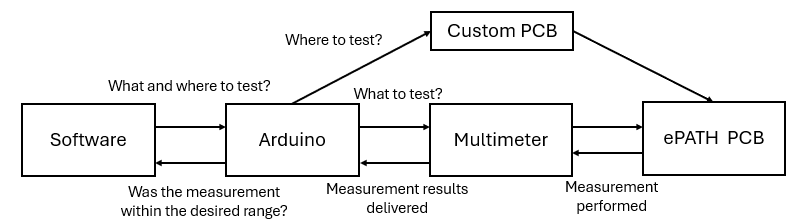
\includegraphics[width=1\linewidth]{img/General end goal diagram.png}
          \caption{Overview of design aspects ePATH testing software.}
          \label{end_goal_diagram}
    \end{figure}

In addition to this some small projects were undertaken. Their individual objectives and achievement are described in the Extra projects subsection.

\subsection{Main Objective}
The specific objectives of ePATH Test Bench project were: 
\begin{itemize}
\item To establish communication between a computer and a multimeter so that any measurements made from the ePATH PCB can easily be processed by the PC to check whether they are as expected.
\item To design a custom PCB board that selects the appropriate pin from the ePATH PCB to be tested. Since the ePATH PCB consists of 2 different grounds, it should accommodate for this by selecting the correct one for each measurement.
\item To develop a GUI that offers an interactive way to do the test.
\item To produce a pdf file with a summary of all the testing results.
\end{itemize}

